%---------------------------------------------------------------------------------------------------
% Hauptteil
%---------------------------------------------------------------------------------------------------
\section{Hauptteil} 

\subsection{Der Token Ring Algorithmus}
Der Token Ring Algorithmus ist ein Wahlalgorithmus der von Chang und Roberts 1979 entworfen wurde. Er kann verteilt auf mehreren Clienten verwendet werden die in einer Ring-Topologie miteinander verbunden sind. Das Ziel des Algorithmus ist, bei Ausfall des Master-Clienten im Netz einen neuen zu wählen.

\subsubsection*{Voraussetzungen}
Damit der Algorithmus auf eine Ring-Topologie angewandt werden kann, müssen folgende Voraussetzungen im Netz gegeben sein:
\begin{itemize}
	\item Jeder Client kennt seinen Nachfolger
	\item Jeder Client ist mit seinem Nachfolger verbunden, sodass er mit ihm kommunizieren kann
	\item Jeder Client hat eine eindeutige ID
	\item Jeder Client kennt die gesamte Ring-Topologie
\end{itemize}

\subsubsection*{Ablauf}
\label{sec:algorithm_process}
Der Algorithmus startet wenn der Master-Client ausfällt. Der Vorgänger des ausgefallenen Master-Clients baut eine Verbindung zum Nachfolger des ausgefallenen Master-Clients auf, sodass die Ring-Topologie wieder vollständig ist.

Der Client, der den Ausfall bemerkt, startet die Wahl in dem er seinem Nachfolger eine Nachricht mit seiner ID und der Info dass es sich um eine Wahl handelt schickt. Dieser nimmt die Nachricht und überprüft ob seine eigene ID darin vor kommt. Falls nicht, hängt er seine eigene ID hinten an und schickt die vervollständigte Nachricht an seinen Nachfolger.

Wenn ein Client feststellt, dass seine eigene ID bereits in der Nachricht vorhanden ist, nimmt er die höchste ID aus der Liste der gesammelten IDs in der Nachricht. Anschließend sendet er eine "Gewählt"-Nachricht mit der höchsten ID an seinen Nachfolger. Der Empfänger der "Gewählt"-Nachricht merkt sich, dass der gewählte Client nun der neue Master ist und sendet seinem Nachfolger die gleiche "Gewählt"-Nachricht. Jeder wird somit benachrichtigt was die höchste ID ist. Kommt die "Gewählt" Nachricht wieder am Initiator der "Gewählt"-Nachricht an, wird die Wahl erfolgreich beendet und der Algorithmus ist terminiert.

\subsubsection*{Eigenschaften}
Die Laufzeit dieses Algorithmus befindet sich in einem Bereich von $0=2N$ wobei N die Anzahl der teilnehmenden Clienten ist. Diese Einschätzung ergibt sich daraus, dass es zwei Nachrichten gibt die jeweils einmal jeden Clienten erreichen müssen. Dabei durchläuft die erste Nachricht, die Wahl N Clienten und die Nachricht, dass ein neuer Master gewählt wurde durchläuft ebenfalls noch einmal N Clienten.
 
Die Eigenschaften des Algorithmus lassen sich so beschreiben
 \begin{itemize}
	\item Laufzeit von 2N
	\item 2 Arten von Nachrichten "Wahl"-Nachricht mit ID Liste und "Gewählt"-Nachricht mit der neuen Master ID
	\item Der Algorithmus findet in einer endlichen Anzahl von Clienten immer den neuen Master (höchste ID)
	\item Alle Teilnehmenden Clienten setzten irgendwann ihren Master auf den gewählten Master 
\end{itemize}
%%Welche Grundlegenden Eigenschaften hat der Algorithmus
%%was tut er und warum, wofür?

\subsection{Spezifikation}
Damit ein Modell erstellt werden kann, das den Algorithmus abbildet, müssen zunächst die charakteristischen Eigenschaften des Algorithmus bestimmt werden.

Der Algorithmus (s. Abschnitt \ref{sec:algorithm_process}) lässt sich in folgende drei Phasen einteilen:
\begin{description}
\item[Phase 1:] Ein Client bemerkt den Ausfall des bisherigen Masters
\item[Phase 2:] Sammeln aller beteiligten Client-IDs
\item[Phase 3:] Bekanntgeben des neuen Masters
\end{description}

Der jeweilige Ablauf der Phasen lässt sich mit folgenden Punkten spezifieren:

\begin{table}
\begin{tabular}{|c|p{7,6cm}|}
\hline Phase & Eigenschaft \\ 
\hline Phase 1: Master-Ausfall bemerkt & Sendet Nachricht zum Wählen und hängt seine eigene ID daran \\ 
\hline \multirow{3}*{Phase 2: Wahl} & Client, der Wahl-Nachricht erhält, hängt seine eigene ID an die Nachricht \\ 
\cline{2-2} & Client sendet die erweiterte Nachricht an seinen Nachfolger \\ 
\cline{2-2} & Sobald ein Client eine Wahl-Nachricht erhält, in der seine eigene ID bereits enthalten ist, geht der Algorithmus in Phase 3 über \\ 
\hline \multirow{3}{*}{Phase 3: Neuen Master mitteilen} & Der Client, der feststellt, dass Phase 2 vorbei ist, sendet eine Nachricht mit dem neuen Master an seinen Nachfolger \\
\cline{2-2} & Ein Client, der die Nachricht über einen Master erhält, merkt sich den neuen Master \\ 
\cline{2-2} & Ein Client, der die Nachricht über einen Master erhält, teilt seinem Nachfolger diese Nachricht mit \\
\cline{2-2} & Sobald der Client, der Phase 3 eingeleitet hat, die Nachricht über den neuen Master erhalten hat, terminiert der Algorithmus \\
\hline 
\end{tabular}
\caption{Spezifikation der Phasen des Algorithmus}
\label{table: algorithm_specification} 
\end{table}

\subsection{Modellierung}

Für die Modellierung wurde der Algorithmus mithilfe der Spezifikation auf seine essentiellen Bestandteile herunter gebrochen und dann an die Möglichkeiten von Petri Netzen angepasst. Es musste ebenfalls verarbeitet werden, das die Möglichkeiten von \textit{Snoopy} hinsichtlich des Umfangs und der Mächtigkeit der Petri Netze eingeschränkt ist. So konnten zum Beispiel die ID Listen in den Nachrichten nicht umgesetzt werden. 


Einige Eigenschaften des Algorithmus bereiten Probleme wenn sie in einem normalen Petri Netz abgebildet werden sollen. Dazu gehört:
 \begin{enumerate}
	\item Clienten haben eine eigene ID
	\item Nachrichten übermitteln unterschiedliche Datenstrukturen (Nachrichten Art, ID Listen)
	\item Bei unterschiedlichen Nachrichten reagiert der Client anders
	\item 
\end{enumerate}

Einige dieser Probleme können dadurch gelöst werden indem ein farbiges Petri Netz genutzt wird (CPN). Dieses ermöglicht mithilfe von Farben und Konstanten jedem Clienten eine eigene ID zu geben. Durch Guards an den Transitionen und Variablen kann ein unterschiedliches Verhalten erzeugt werden. Ein Problem das sich damit allerdings nicht lösen lies war die Datenstrukturen. Ein Token kann nur einen einzigen Wert haben.

Um dieses Problem zu beheben wurde der Algorithmus ein wenig verändert. Für die Modellierung werden keine ID Listen weiter gereicht sondern nur noch eine einzige ID und zwar die Lokal größte. Das bedeutet der Initiator schickt seine ID zu seinem Nachbarn. Dieser vergleicht die ID mit der eigenen und schickt die Größere weiter. Dies stellt keine Grundlegende Änderung in der Funktionsweise des Algorithmus dar sondern verschiebt bloß den Schritt des Vergleichs. Nun überprüft nicht mehr nur der Initiator welches die höchste ID ist, sondern jeder Client überprüft die eigene ID mit der empfangenen. Wie der Algorithmus nun im Detail abläuft wird im Folgenden beschrieben.

Um den Algorithmus abzubilden wurde ein farbiges Petri Netz gewählt um den Token eine Gewichtung geben zu können die die ID der jeweiligen Clienten widerspiegelt. Des Weiteren war es notwendig an den Transitionen entscheiden zu können wann diese Schalten. Auch dies bietet das farbige Petri Netz (CPN) durch Guards.

%%Wie haben wir ihn modelliert
%%-Gefärbtes netz
%%- Ids
%%- Guards
%%Erklären an wo die spezifizierten Punkte im Netz zu finden sind.

\subsubsection{Das Netz}
Hier Netzbild einbinden
\begin{figure}[H]
\centering
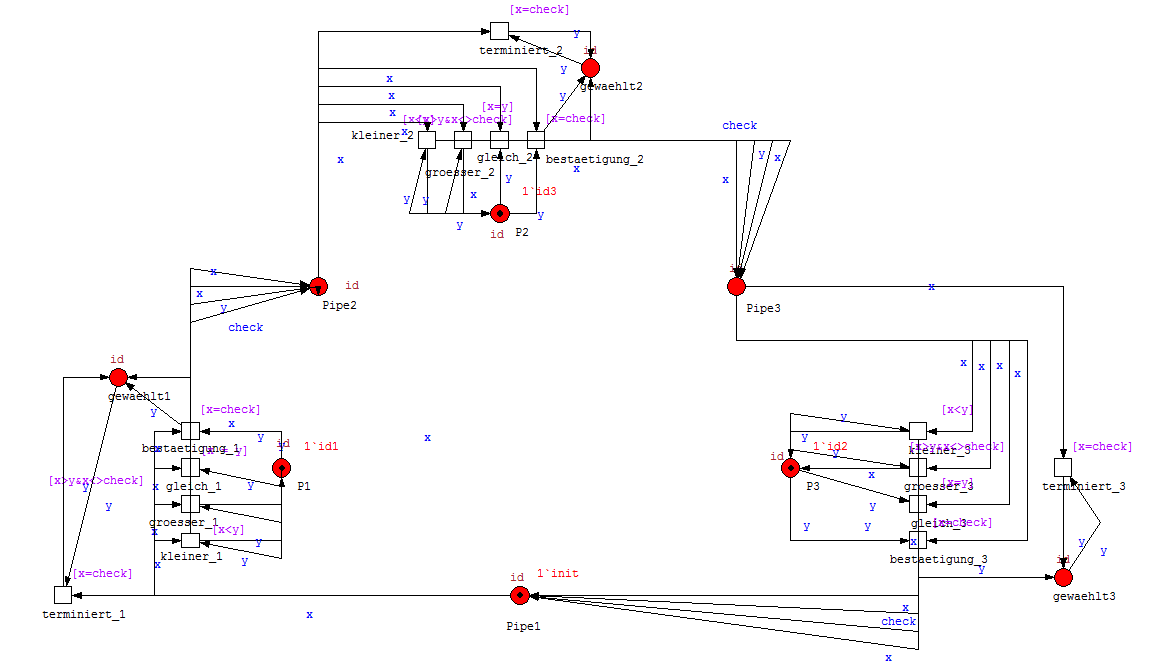
\includegraphics[width=1\linewidth]{./cpn}
\caption{Der Token Ring ALgorithmus als farbiges Petri Netz}
\label{fig:cpn}
\end{figure}

\begin{figure}[H]
\centering
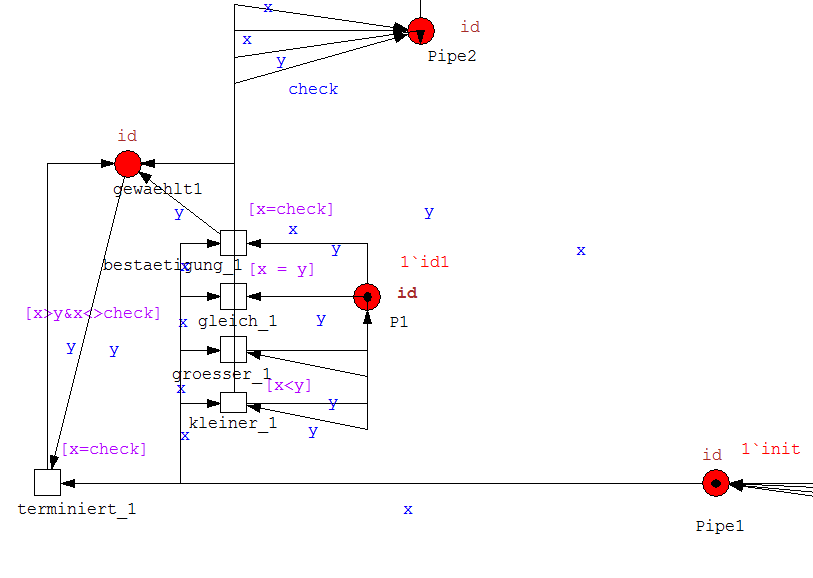
\includegraphics[width=1\linewidth]{./cpn_detail}
\caption{Detailausschnitt eines Clienten}
\label{fig:cpn_detail}
\end{figure}



\subsection{Korrektheit}
Warum ist der Algorithmus korrekt
- Determinismus
- es kann immer nur eine Transition schalten es gibt keine Parallelität
- Erreichbarkeitsgraph zeigen und erklären
